\section{Implementation}\label{sec:architecture}
In this section dedicated to the implementation of the thesis' code, we will delve into the organizational framework of the foundational code derived from the GitHub repository \cite{LFighter_code}. We will discuss the structural elements that constitute the basis of our work, elucidating the positioning of the newly crafted code that serves the thesis' purpose. The goal is to demonstrate how the intricate nature of a typical FL environment is mirrored in the architecture of this implementation by drawing comparisons to real-world FL scenarios and the base code structure.

We will also dive deep into our label flipping algorithms using a methodical approach that starts with a study of the base code dissected in Section \ref{sec:base_code}. In order to lay the foundation for our hypotheses, this first step involves disassembling the existing components and exploring the rationale behind their design decisions.

The proposed hypotheses, which range from new ideas to small modifications, collectively aim to refine and enhance the overall performance of the label flipping attacks. Through careful implementation and rigorous testing, we seek to demonstrate the efficacy of our approach and highlight the evolution of label flipping algorithms into more sophisticated and effective tools for adversarial scenarios. The implemented code can be accessed on the project's GitHub repository \cite{MastersThesisCode}.

For the upcoming results, which will be detailed in Section \ref{sec:results}, our focus revolves around devising attacks that optimize four parameters:
\begin{itemize}
        \item Test error (TE). Error resulting from the loss function used in training. The lower TE, the better.
        \item Overall accuracy (All-Acc). Number of correct predictions divided by the total number of predictions for all the examples. The greater All-Acc, the better.
        \item Source class accuracy (Src-Acc). Number of the source class examples correctly predicted divided by the total number of the source class examples. The greater Src-Acc, the better.
        \item Attack success rate (ASR). Proportion of the source class examples incorrectly classified as the target class. Since we aim to attack the system, the higher ASR, the better.
\end{itemize}

%%%%%%%%%%%%%%%%%%%%%%%%%%%%%%%%%%%%%%%%%%%%%%%%%%%%%%%%%%%%%%%%%%%%%%%%%%%%%%%%%%%%%%%%%%%%%%%
\subsection{Base code structure} \label{sec:base_code}
The base code is implemented in Python and structured as follows:
\begin{itemize}
        \item Python notebooks (.ipynb files): There are three notebooks, one for each dataset used in the developer's experiments. The included datasets are:
        \begin{itemize}
                \item MNIST \cite{MNIST}: This dataset contains samples of handwritten digits. It consists of a training set of 60,000 samples, and a test set of 10,000 samples. Each sample is a 28x28 bit grayscale image, associated with a label from 10 classes. The task is to classify the images into their respective digit classes.
                \item CIFAR-10 \cite{CIFAR10}: This dataset contains 60,000 32x32 bit colour images in 10 different classes. These classes encompass a diverse array of objects, including but not limited to animals, vehicles, and everyday items. The objective underlying this dataset is to accurately classify each image into its designated class.
                \item IMDB \cite{IMDB}: This dataset contains 50,000 movie reviews from the Internet Movie Database. The task is to classify the reviews into positive or negative sentiment.
        \end{itemize}
        The notebooks are used to run the experiments using the different aggregation functions commented in section \ref{sec:aggregation_methods} at user's will. This is done by importing the libraries and defining global variables in one executable section, and arranging the tests with different aggregation methods into separate sections. These notebooks are also used to visualize the results and checking the process.
        \item \textit{experiment\_federated.py}: This python file contains a sole function (\textit{run\_exp()}) that is called by one of the Python notebooks whenever we wish to start a new experiment with an aggregation function. This function merely prints by console information concerning the parameters used in the current experiment, initializes the FL environment, and calls a more complex function.
        \item \textit{environment\_federated.py}: This is the most complex file in the base code. It contains the \textit{run\_experiment()} function, which is the one called by the previous file. This function is responsible for the execution of the experiment, and it is where the whole FL setting is initialized and simulated. The file is divided into two main classes:
        \begin{itemize}
                \item Peer: When a Peer object is created, the Peer class initializes all its variables, such as the peer's ID, its local data, etc. This class contains a single function, named \textit{participant\_update()}, which is called when a peer has to update its local model. This function is responsible for the training of the local model, and it is where, depending on the value of the parameter "\textit{attack\_type}", the execution of the attack is determined. The function returns the updated local model.
                \item FL: This class is responsible for the initialization of the FL environment, from the most simple parameters such as the global rounds, to the more complex tasks such as creating the peers' instances and setting the global model up. It contains four functions:
                \begin{itemize}
                        \item \textit{test()}: This function is used to test the model's accuracy.
                        \item \textit{test\_label\_predictions()}: As the name suggests, this function is used to test the label predictions of the model received as a parameter. It is responsible for returning a list with the actual labels and another with the predicted ones in order to obtain the accuracy of the model.
                        \item \textit{choose\_peers()}: This function selects \textit{n} random peers from the list of peers. The value of \textit{n} is determined by the total amount of peers and the malicious rate, which is a floating-point variable.
                        \item \textit{run\_experiment()}: This is the function that simulates the whole FL environment. The function is built as follows:
                        \begin{enumerate}
                                \item It begins by copying the global model into a local variable.
                                \item After that, it iterates through a loop a total of "\textit{global\_rounds}" times. Inside this loop, for each global round, it selects the peers that will participate in the current round by calling the \textit{choose\_peers()} function, it also reinitializes the utility tables (weights, local models, etc.) of the peers that will participate in the current round, and then, for each peer participating:
                                \begin{enumerate}
                                        \item It defines the peer as attacker or regular depending on the output of \textit{choose\_peers()}, calls the \textit{participant\_update()} function of the peer.
                                        \item It updates the utility tables of the peer with the new values.
                                \end{enumerate}
                                \item After all peers have been updated, it aggregates the local models of the peers that participated in the current round by the selection of the aggregation function dependant on a series of conditional statements.
                                \item It updates the global model with the aggregated model and the process is repeated until the global rounds are completed.
                                \item The \textit{test()} function is called to obtain the model's accuracy.
                                \item Finally, it returns the system's state by console.
                        \end{enumerate}
                \end{itemize}
        \end{itemize}
\end{itemize}
The logical location for the hypotheses code is inside the \textit{environment\_federated.py} file. The exact placement for these functions is inside the \textit{participant\_update()} function, contained by the Peer class.
This is because it is the single point of entry for the execution of the attack, and it is where the local model is updated.


\subsection{Real-world FL vs. base code}
In this section, we state the similarities between a real FL system and the base code described in the previous section, \ref{sec:base_code}. As an aid as we navigate through the details of these two distinct environments, \autoref{fig:FL_diagram} provides a diagram of an actual FL scenario to further illuminate this comparison. 
\begin{figure}[h]
        % \begin{figure}[H] % Alternative positioning
        \centering % sempre
        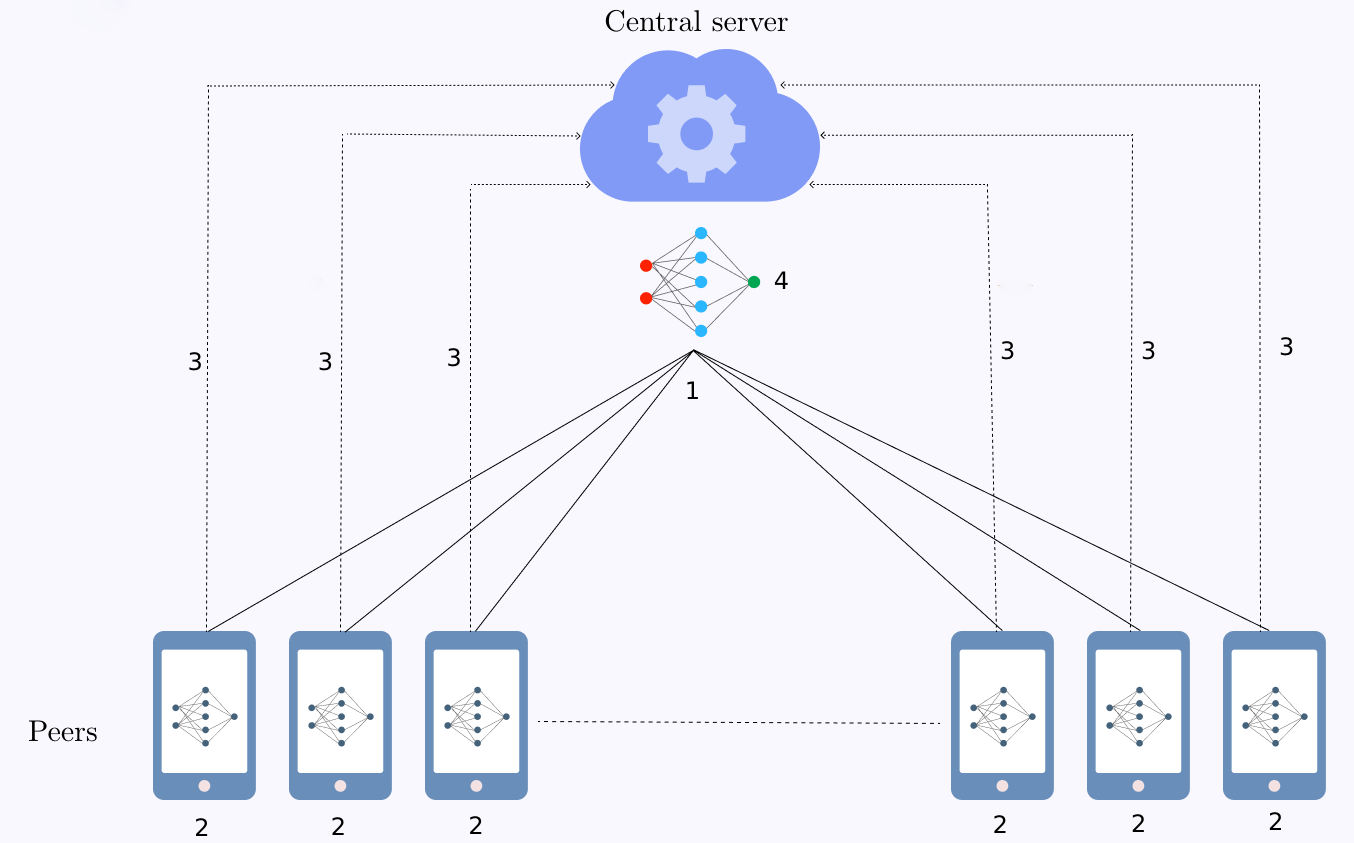
\includegraphics[scale=0.3]{FL_diagram.png}
        \caption{Federated Learning process. Source: \textit{Devfi}} % sempre
        \label{fig:FL_diagram}
\end{figure}

Next, the steps comprising the diagram are briefly outlined:
\begin{enumerate}
        \item The server sends the global model to the clients. This step is mirrored in the base code at the beginning of the \textit{run\_experiment()} function, which is responsible for the initialization of the FL environment, and it is where the global model is initialized and sent to the clients.
        \item The clients train the model with their local data. The second step exhibits its equivalence in the \textit{participant\_update()} function, which is called for each peer participating in the current round. This function is responsible for the training of the local model.
        \item The clients send the updated models to the server. This step is difficult to locate in the base code, as it is not explicitly stated. However, it is possible to infer that the updated models are sent to the server in the \textit{run\_experiment()} function, where the local models are located in table structures managed by the code.
        \item The server aggregates the models and sends the updated global model to the clients. This step is mirrored in the base code at the series of if statements mentioned in the previous section, \ref{sec:base_code}, which are responsible for the aggregation of the local models.
\end{enumerate}
The process is repeated until the global model converges. This step is mirrored in the loop defined in the \textit{run\_experiment()} function, which is dependent on the value of the parameter "\textit{global\_rounds}".


%%%%%%%%%%%%%%%%%%%%%%%%%%%%%%%%%%%%%%%%%%%%%%%%%%%%%%%%%%%%%%%%%%%%%%%%%%%%%%%%%%%%%%%%%%%%%%%
\subsection{Chosen parameters and modifications}\label{sec:chosen_parameters}
The first step after dissecting the base code \cite{LFighter_code} is to choose the parameters that we use for our experiments:
\begin{itemize}
        \item Independent and Identically Distributed (IID) data: In an IID case, all the peers have a uniform sample of the data, meaning each peer possesses a similar proportion of each class. Thus, each of them represents a proportion of the global data. As a result, every update they compute serves as an unbiased estimate of the global model. In the non-IID scenario, this is not the case. Each user could have different percentages of classes or contain a lot of outliers or various other scenarios. In the most extreme case, each user might only have data corresponding to a single class. In such instances, the updates computed by peers can be significantly dissimilar from one another. 
        
        IID is the simpler case for defences, and therefore more challenging for attackers. If an attack performs moderately well in the IID case, it should perform better in the non-IID case. Or, at the very least, it should be harder to detect. That is why it makes sense to start here. The non-IID case would be the most favourable scenario, as many defences will likely fail directly. The reality is that peers typically fall somewhere in between: neither fully IID nor completely non-IID. The IID case serves as a good starting point for research into these topics.
        \item Global rounds: This variable is set to 100. This means that the global model is updated 100 times.
        \item Local epochs\footnote{Epochs refer to the quantity of iterations a ML algorithm performs on the entire training dataset. Each epoch involves the algorithm making incremental adjustments to its model parameters based on the training data, aiming to improve its performance over time.}: This variable is set to 3. This means that each peer trains its model for 3 epochs before sending the update to the server.
        \item Number of peers: There are 20 peers in the system. 
\end{itemize}

Another minimal change made to the base code is adding a condition to check if the device being used for the experiments is a Graphics Processing Unit (GPU) or the device's Central Processing Unit (CPU). This change is made because the GPU is much faster than the CPU when employing tensors\footnote{Tensors are multi-dimensional arrays commonly used in mathematics and ML to represent data. In ML, tensors are used to store and manipulate data, such as images, sequences, and more complex structures. Tensors are particularly well-suited for ML tasks due to their ability to efficiently handle large volumes of data and perform operations in parallel. GPUs are highly effective for tensor operations, as they are optimized for parallel computing.}. The code used to perform this check is shown in \autoref{listing:gpu_check}.

\begin{listing}[h]
        \begin{minted}
        [
            autogobble,
            breaklines,
            breakautoindent,
            % highlightlines={1, 3-4},
            linenos
        ]
        {python}
        import torch
        ...
        if torch.cuda.is_available():
                DEVICE = "cuda"
                print('GPU is available:', torch.cuda.get_device_name(0))
        else:
                DEVICE = "cpu"
                print('GPU is not available, CPU will be used')
        DEVICE = torch.device(DEVICE)
        ...
        \end{minted}
    
        \caption{Computing device selection and information}
        \label{listing:gpu_check}
    \end{listing}

Finally, we also added a section after the FL system has finished the global rounds to print the results obtained in a confusion matrix format. This matrix is a table that is often used to describe the performance of a classification model on a set of test data for which the true values are known. The code used to print this matrix is shown in \autoref{listing:confusion_matrix_code}.

\begin{listing}[h]
        \begin{minted}
        [
            autogobble,
            breaklines,
            breakautoindent,
            % highlightlines={1, 3-4},
            linenos
        ]
        {python}
        from matplotlib import pyplot as plt
        ...
        actuals, predictions = self.test_label_predictions(simulation_model, self.device, self.test_loader, dataset_name=self.dataset_name)
        plt.matshow(confusion_matrix(actuals, predictions))
        plt.colorbar()
        plt.show()
        ...
        \end{minted}

        \caption{Printing the confusion matrix}
        \label{listing:confusion_matrix_code}
\end{listing}

\subsection{Implementation of the entropy-based label flipping attack}
The code that implements the entropy-based label flipping attack and serves as a reference for other attacks implemented is shown in \autoref{listing:entropy_label_flipping_code}.

As commented in Section \ref{sec:entropy_label_flipping}, there is a need for a new function that serves the purpose of flipping the labels of the samples that are going to be poisoned. This function is called \textit{index\_label\_flip()} and is shown in \autoref{listing:index_label_flip_code}.

Given that the execution time for an attack with the parameters mentioned in Section \ref{sec:chosen_parameters} is approximately 4 hours for an Nvidia RTX2060 graphics card, and that we are executing eight attacks per poisoning method, as seen in Section \ref{sec:defenses}, we are not able to try all the possible modifications of the entropy-based label flipping attack. Therefore, we have to choose the ones that we think are the most promising. 
The modifications that we have chosen to implement and test are the following:
\begin{itemize}
        \item Keeping the highest 25\% entropies. This modification is based on the idea that the samples with the highest entropy are the ones that are more likely to be misclassified. Therefore, if we are more specific and only flip the labels of the samples with the highest entropy, we should be able to increase the attack success rate by avoiding detection from the server. To modify the code, we only have to change line 23 of \autoref{listing:entropy_label_flipping_code} to \textit{num\_elements\_to\_keep = len(sorted\_entropy\_list) // \textbf{4}}.
        \item Keeping the highest 75\% entropies. This modification is based on the opposite idea, that is, if the attack is avoiding detection when poisoning 50\% of the samples, we can try to increase the attack success rate by poisoning more samples.
        \item Keeping the lowest 50\% entropies. The thought for this idea is that the samples with the lowest entropy are the ones that are easier to classify. Therefore, if we flip these labels, we may be able to confuse the server in the first training rounds, and indirectly lean benevolent peers to misclassify the samples according to our will. To modify the code, we only have to change line 22 of \autoref{listing:entropy_label_flipping_code} to \textit{sorted\_entropy\_list = sorted(entropy\_list, key=lambda x: x[1], reverse=\textbf{False})} so the list is ordered by ascending entropy.
        \item Keeping the lowest 25\% entropies. The reason for this modification is the same as the previous one, but being more specific and only flipping the labels from the samples that better represent the source class.
        \item Applying a scaling factor to the weights before the update. This modification is based on literature proposals to ensure a successful attack, commented in Section \ref{sec:defenses}. The code used to implement this modification is shown in \autoref{listing:scaling_factor_code}. The code is located at the end of the \textit{participant\_update()} function to receive the trained local model.
\end{itemize}

\begin{listing}[H]
        \begin{minted}
        [
            autogobble,
            breaklines,
            breakautoindent,
            % highlightlines={1, 3-4},
            linenos
        ]
        {python}
        if (attack_type == 'entropy_label_flipping') and (self.peer_type == 'attacker'):
            train_loader = DataLoader(self.local_data, self.local_bs, shuffle = False, drop_last=True)
            model.eval()  # Set the model to evaluation mode
            entropies = []  # To store entropies for each data sample
            kept_indices=[] #to store the indices of the data samples with label==target_class
            with torch.no_grad():
                for batch_idx, (data, labels) in enumerate(train_loader):
                    # Find the indices of data samples with label of the source class
                    source_mask = labels == source_class
                    # Keep the positions of the data samples with label==source_class
                    kept_indices_batch = (batch_idx * train_loader.batch_size + i for i in range(len(source_mask)) if source_mask[i])
                    kept_indices.extend(kept_indices_batch)
                    # Get the data samples with label target
                    data_source_batch = data[source_mask]
                    # Send the data samples with label=source_class to the device
                    data_source_batch = data_source_batch.to(self.device)
                    # Obtain the predicted outputs for data samples with label source_class
                    output = model(data_source_batch)  # Get the model's output for the source class data samples
                    predictions_np=(output.cpu().numpy())   # Convert the output to numpy
                    entropies.extend(stats.entropy(predictions_np, axis=1)) # Entropy is calculated by row
            entropy_list = list(zip(kept_indices, entropies))
            sorted_entropy_list = sorted(entropy_list, key=lambda x: x[1], reverse=True)    # Sort it by entropy value
            num_elements_to_keep = len(sorted_entropy_list) // 2   # Number of elements that represents the 50% of the data that we can attack
            top_50_percent = sorted_entropy_list[:num_elements_to_keep] # Extract the top 50% of the data
            sorted_entropy_list = sorted(top_50_percent, key=lambda x: x[0])  # Sort by index to keep the order of the data
            
            poisoned_data = index_label_flip(train_loader.dataset, sorted_entropy_list, target_class)
            # Create a new DataLoader with the updated dataset and with a shuffle
            train_loader = DataLoader(poisoned_data, self.local_bs, shuffle = True, drop_last=True)
            self.performed_attacks+=1
            print('Entropy-based Label flipping attack launched')
        \end{minted}

        \caption{Entropy-based label flipping algorithm}
        \label{listing:entropy_label_flipping_code}
\end{listing}

\begin{listing}[H]
        \begin{minted}
        [
            autogobble,
            breaklines,
            breakautoindent,
            % highlightlines={1, 3-4},
            linenos
        ]
        {python}
        def index_label_flip(dataset, sorted_list, target_class):
                poisoned_data = []
                for i, (data, label) in enumerate(dataset):
                if i in [index for index, _ in sorted_list]:
                        poisoned_data.append((data, target_class))  # Change the label to target_class
                else:
                        poisoned_data.append((data, label))  # Keep the original label
                return poisoned_data
        \end{minted}

        \caption{\textit{index\_label\_flip()} function}
        \label{listing:index_label_flip_code}
\end{listing}

\begin{listing}[H]
        \begin{minted}
        [
            autogobble,
            breaklines,
            breakautoindent,
            % highlightlines={1, 3-4},
            linenos
        ]
        {python}
        def scale_model(update, scale_factor):
                for key in update.keys():
                update[key] = (update[key].float() * scale_factor).long()
                return update
        ...
        if self.peer_type == 'attacker' and (attack_type == 'entropy_label_flipping' or attack_type == 'closeness_label_flipping'):
                update = scale_model(model.state_dict(), scale_factor = 1.1)
                model.load_state_dict(update)
        \end{minted}

        \caption{Scaling factor implementation}
        \label{listing:scaling_factor_code}
\end{listing}

The verification process to ensure the correct functionality of the entropy-based label flipping algorithm has been carried out with meticulous attention to detail. Extensive testing and validation procedures have been executed to ensure that the algorithm operates as intended. The different evaluations that have been used to evaluate the algorithm's behaviour and performance are listed below:
\begin{itemize}
        \item Printing the entropies list to ensure that the range of values is correct. Then, printing the length of the entropies list and the indices list to ensure that they have the same length.
        \item Printing the sorted entropy list to ensure that the list is sorted by descending entropy. Then, when the list is trimmed, printing it again to make sure it is ordered by index.
        \item Counting and printing the amount of source class labels before and after the poisoning to ensure that the number of samples with the source class label has been reduced by the number of elements in the sorted entropy list. Then, performing the same operation with the target class label to ensure that the number of samples with the target class label has been increased by the number of elements in the sorted entropy list.
\end{itemize}




\subsection{Implementation of the closeness-based label flipping attack}
The implementation of the closeness-based label flipping attack is very similar to the entropy-based label flipping attack. The code that implements the closeness-based label flipping attack is shown in \autoref{listing:closeness_label_flipping_code}.

The set of different modifications that we have chosen to implement and test for the closeness-based label flipping attack are the following:
\begin{itemize}
        \item Keeping the highest 25\% closeness. This modification is based on the idea that the samples with the highest closeness are the ones that are more likely to be misclassified as the target class.
        \item Applying a threshold instead of keeping a percentage. The rationale behind this modification is that, as the global rounds progress, the global model is more refined. Therefore, the top percentage may include samples that are not as close to the target class as they were in the first global rounds. In order to mitigate this, we can try to keep the samples with a closeness difference, lower than a threshold. The code used to implement this modification is shown in \autoref{listing:threshold_code}. The code is located before the call to the \textit{index\_label\_flip()} function.
\end{itemize}


\begin{listing}[h]
        \begin{minted}
        [
            autogobble,
            breaklines,
            breakautoindent,
            % highlightlines={1, 3-4},
            linenos
        ]
        {python}
        if (attack_type == 'closeness_label_flipping') and (self.peer_type == 'attacker'):
        ...
        closeness = []  # To store entropies for each data sample
        kept_indices=[] #to store the indices of the data samples with label==target_class
        with torch.no_grad():
        ...
                predictions_np=(output.cpu().numpy())   # Convert the output to numpy
                temp = []
                for i in range(len(predictions_np)):
                        temp.append(abs(predictions_np[i][source_class] - predictions_np[i][target_class]))
                closeness.extend(temp)
        ...
        \end{minted}

        \caption{Closeness-based label flipping algorithm}
        \label{listing:closeness_label_flipping_code}
\end{listing}
\begin{listing}[h]
        \begin{minted}
        [
            autogobble,
            breaklines,
            breakautoindent,
            % highlightlines={1, 3-4},
            linenos
        ]
        {python}
        ...
        sorted_closeness_list = sorted(closeness_list, key=lambda x: x[1])    # Sort it by entropy value
        threshold=0.02
        count=1
        actual=sorted_closeness_list[0][1]
        while actual <= threshold and count < len(sorted_closeness_list):
                count += 1
        num_elements_to_keep = count   # Number of elements that to keep
        top_closeness = sorted_closeness_list[:num_elements_to_keep]
        ...
        \end{minted}

        \caption{Threshold implementation}
        \label{listing:threshold_code}
\end{listing}
The verifications to test the correct functionality of the closeness-based label flipping algorithm are the same as the ones used for the entropy-based label flipping algorithm.


\subsection{Implementation of the adaptive label flipping attack}
As described in Section \ref{sec:adaptive_label_flipping}, the adaptive label flipping attack is a combination of using the entropy-based or closeness-based label flipping attacks, while flipping a different number of labels depending on the global round the system is in. The code that implements the adaptive label flipping attack is shown in \autoref{listing:adaptive_label_flipping_code}.

\begin{listing}[H]
        \begin{minted}
        [
            autogobble,
            breaklines,
            breakautoindent,
            % highlightlines={1, 3-4},
            linenos
        ]
        {python}
        if (attack_type == 'stealthy_closeness_label_flipping') and (self.peer_type == 'attacker'):
                ...
                if global_epoch > 25:
                        with torch.no_grad():
                                ...
                        sorted_entropy_list = sorted(entropy_list, key=lambda x: x[1], reverse=True)
                        num_elements_to_keep=0
                        if global_epoch <= 50:  # round 25 to 50, flip 75% of the data
                                num_elements_to_keep = len(sorted_entropy_list) // 2 + len(sorted_entropy_list) // 4
                        if global_epoch <= 75:  # round 50 to 75, flip 50% of the data
                                num_elements_to_keep = len(sorted_entropy_list) // 2
                        if global_epoch <= 100: # round 75 to 100, flip 25% of the data
                                num_elements_to_keep = len(sorted_entropy_list) //4
                        ...
                else:   # round 0 to 25, flip all the data
                        poisoned_data = label_filp(self.local_data, source_class, target_class)
                        train_loader = DataLoader(poisoned_data, self.local_bs, shuffle = True, drop_last=True)
                ...
        \end{minted}
        \caption{Adaptive label flipping algorithm}
        \label{listing:adaptive_label_flipping_code}
\end{listing}
The first segment does not follow the usual code because, since all the labels are flipped there is no point in computing the entropy or the closeness of the samples.

The set of different modifications that we have chosen to implement and test for the adaptive label flipping attack are the following:
\begin{itemize}
        \item Testing with entropy and closeness-based label flipping to  flip all the labels during the first half of the global rounds. During the second half, flip 50\% of the samples.
        \item Testing with either entropy or closeness-based label flipping to flip all the labels during the first half of the global rounds. During the second half, flip 25\% of the samples.
\end{itemize}

The verifications to test the correct functionality of the adaptive label flipping algorithm are the same as the ones used for the previous label flipping algorithms.






\pagebreak